\documentclass[a4paper]{scrartcl}
\usepackage[utf8]{inputenc}
\usepackage[english]{babel}
\usepackage{graphicx}
\usepackage{lastpage}
\usepackage{pgf}
\usepackage{wrapfig}
\usepackage{fancyvrb}
\usepackage{fancyhdr}
\pagestyle{fancy}
\usepackage{dingbat}

\usepackage[autostyle]{csquotes}
\usepackage[
    backend=biber,
    style=ieee,
    sortlocale=de_DE,
    natbib=true,
    url=true,
    doi=true,
    eprint=false
]{biblatex}
\addbibresource{id1354-report-template.bib}

\usepackage[]{hyperref}
\hypersetup{
    colorlinks=true,
}

% Create header and footer
\headheight 27pt
\pagestyle{fancyplain}
\lhead{\footnotesize{Internet Applications, ID1354}}
\chead{\footnotesize{Seminar 3}}
\rhead{}
\lfoot{}
\cfoot{\thepage\ (\pageref{LastPage})}
\rfoot{}

% Create title page
\title{Seminar 3}
\subtitle{Internet Applications, ID1354}
\author{Jacob Kimblad, jacobki@kth.se}
\date{1019-01-08}

\begin{document}

\maketitle

\section{Introduction}

The third seminar deals only with non-functional requirements but is instead all about improving the structure of the PHP and appication in general. The main idea is to restructure the application produced for seminar 1 and seminar 2 into a Model-View-Controller (MVC) structure. This can be done manually by restructuring all of the code into new folders and refactoring the code appropriately. 
Another option is to use an existing framework that provides a MVC structure for web-applications. Provided in the assignment are some rules to make sure the application follows the MVC structure and also has low coupling and high cohesion, these rules are summarised below.

\begin{itemize}
    \item No HTTP or HTML outside of the view layer.
    \item Nothing displayed on screen should be generated outside the view layer. 
    \item Nothing related to databases outsed the integration layer.
    \item No logic outside the integration layer.
\end{itemize}

To solve this task the author has chosen to go with the option to use an existing PHP Framework. The requirements provided in the assigment for this task is summarised below.

\begin{itemize}
    \item The framwork must make the web application follow the MVC architectural pattern.
    \item The framework must be used to split the application into layers which all have the roles specified by MVC.
    \item All PHP code in the controller and the model, as well as much as possible in the view, must be object-oriented.
    \item Duplicated code must be avoided.
\end{itemize}

In addition to restructure the code to follow the MVC architectural pattern the author is also expected to implement some security features on the webpage to handle malicious users. The assignment provides the option to implement three safety feature freely picked from a list of six. This list presented in the assigment is provided below.

\begin{itemize}
    \item File system security.
    \item Input Filtering.
    \item Dabase security (if applicable).
    \item Password encryption.
    \item Cross site scripting.
    \item Impersonation.
\end{itemize}

In addition to these requirements the author is also expected to present a class diagram to illustrate the application.

\section{Literature Study}
Codeigniter version 3, which is the chosen PHP framework, have extensive online documentation that can be found at \citet{noauthor_codeigniter_docs}. This will probably be used frequently by the author during development. The youtube channel Traversy Media also has a series of videos \citet{noauthor_youtube_nodate} walking through how to build a blogging website using PHP and Codeigniter implementing a lot of the same functionality as this assigment. The main source of information will probably be gathered from the youtube series.

This section must prove that you collected sufficient knowledge before starting development, instead of just hacking away without knowing how to complete the task. State what you have read and briefly summarize what you have learned.

\section{Method}

In addition to the LAMP stack setup during the last seminar the author also used a PHP framework known as Codeigniter \citet{noauthor_codeigniter_nodate} during this assignment. The LAMP stack is built using Arch Linux, Apache web server, MariaDB and PHP. For editing files VIM is used. The main browser used by the author is Firefox, which will be the browser used mainly for testing during development. Other browsers such as Chromium and online browser tools will be used before release. The mozilla CSS and HTML checkers are used to verify both the HTML and the CSS of the application to remove any errors and possible warnings.  

\section{Result}

As can be seen from the folder structure under the application folder in the Github repository \citet{kimblad_git_2019} there exists a separate folder vor views, controllers and models. There are also additional folders that are provided by Codeigniter that enables different configurations and libraries to be used with the framework. The class diagram can be seen in figure \ref{fig:class_diagram}.

\subsection{Views}
The views folder consists strictly of files with HTML that are intended to be viewn as web-pages. These include the pancake and meatball recipe pages, a login and register page for handling users, a footer and header that are place above and below the rest of the pages as well as the calendar, home and about pages.

\subsection{Controllers}
The view layer contains all of the HTML code and some additional PHP code. The PHP code is mostly used to display HTML depending on if a user is logged in or not using a session variable provided by Codeigniter \citet{kimblad_git_2019-session}.
It is also used to create forms using a form helper provided by Codeigniter. This makes it such that small parts of the PHP code is not object oriented, as it would only serve to increase the complexity of the code by hiding simple code that is only used one time behind class functions and a need for very many class functions. It is also required that no HTML code is generated from outside the view layer and passed in, which in many cases makes it easier to have one or two lines of simple to understand PHP inside the view to get the job done.
Example of PHP code in the view layer is when comments are displayed, as these needs to be fetched from the database the PHP code in the view need to contact the right controller as can be seen at \citet{kimblad_git_2019-1} where the variable containing the comments is provided by a controller that speaks with the model layer. 

The controller layer contains logic that is used by php in the view layer when the user is interacting with the website during normal usage. There are three controllers defined for this assignment, Comments, Pages and Users. The Comments controller has two functions, create and delete. 
Create serves to create a new comment that has been defined by the logged in user and send the apropriate information to the model, which stores it in the database and on the contrary delete serves to delete a comment selected and made by the logged in user. 

The Pages controller serves pages to the users web browser and helps to avoid duplicated HTML code by using a provided template for the header and footer of the page. This means that the navbar only needs to be written once into its own HTML document which is then loaded at the top of the page above the unique page that the user is visitng. 

The Users controller handles all of the necessary logic to have a user register, log in and log out. This controller includes functions register, login, logout and check\_username\_exists.
The register function sends a username and associated hashed password to the user model. The login function sends a username and password pair to the user model and if the exists as a registered user the user is saved in the Codeigniter session variable as logged in.
The logout function unsets all of the previoiusly saved data in the codeigniter session variable.
The check\_username\_exists function contacts the user model with a username and which returns if the username exists as a registered user or not.

\subsection{Models}
There are two classes to be found in the model layer, the Comment\_model and User\_model. Each model is connected to the MariaDB and fetches and stores information in a single table. The Comment model has three functions, get\_comments which fetches all comments existing in the database (as figuring out the relevant one is the controllers assignment), create\_comment inserts a new comment, associated username and relevant page as a new row into the database and delete\_comment removes a comment in the database given its id.

The user model consists of three functions, register insterts a new username and encrypted password into the "Users" table in the database, login returns the rows that are associated with the username and password pair that was provided and check\_username\_exists is used by the controller to check if a username is already registered in the database.

\begin{figure}[h!]
  \begin{center}
    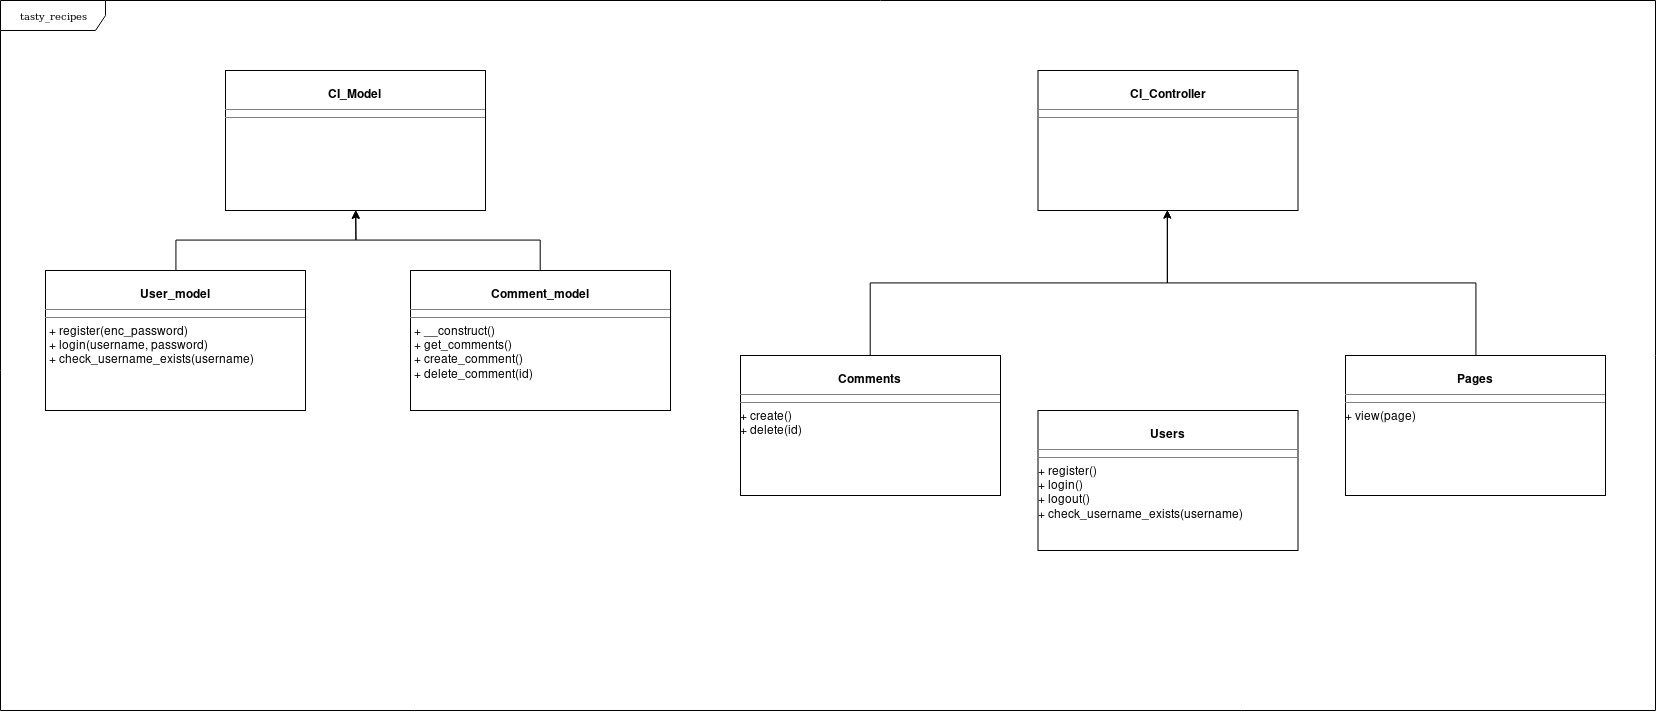
\includegraphics[scale=0.25]{images/class_diagram.png}
    \caption{Class diagram of the application.}
    \label{fig:class_diagram}
  \end{center}
\end{figure}

\subsection{security}
Password encryption was implemented by using the md5 hash algorithm built into the PHP standard library. The password is hashed before it is stored in the database, such that no clear-text passwords are stored. Instead of the actual password being compared when logged in we compare the hash of the inputted password to the hash in the database to see if there is a match. The password is hashed here \citet{kimblad_git_2019-2}.

Input filtering is automatically provided for controllers in Codeigniter using the input class. This class makes sure to pre-process any input data on the page for security. The documentation for the input class can be found here \citet{codeignite}.

Cross site scripting is also a feature that is built into Codeigniter. It is easily turned on by enabling it in a config file that can be found here \citet{cxx}. This makes it such that evertime a GET, POST or COOKIE is encountered the cross site scripting filter is enabled automatically.

\section{Discussion}

The author has shown for the requirements to be completed as no HTML exists outside of the views, everything displayed on the screen is generated within the views, noting related to databases or any logic outside of the integration layer. The requirements specific to the task of using an existing framework are also met as the framework devides the application up in an MVC architecure, all PHP code in the model and controller is object-oriented and duplicated code is avoided.
For the requirements regarding security it has been shown that the site uses password encryption, input filtering and also is safe against cross site scripting.
One lesson is that the used hashing algorithm md5 is no longer considered secure and other existing options should be used instead.


\printbibliography

\section{Comments About the Course}
The author spent approximately 40 hours on this assignment.

\end{document}
